\chapter{Hiểu về Node - Đơn vị cơ bản của n8n}

\begin{figure}[htbp]
    \centering
    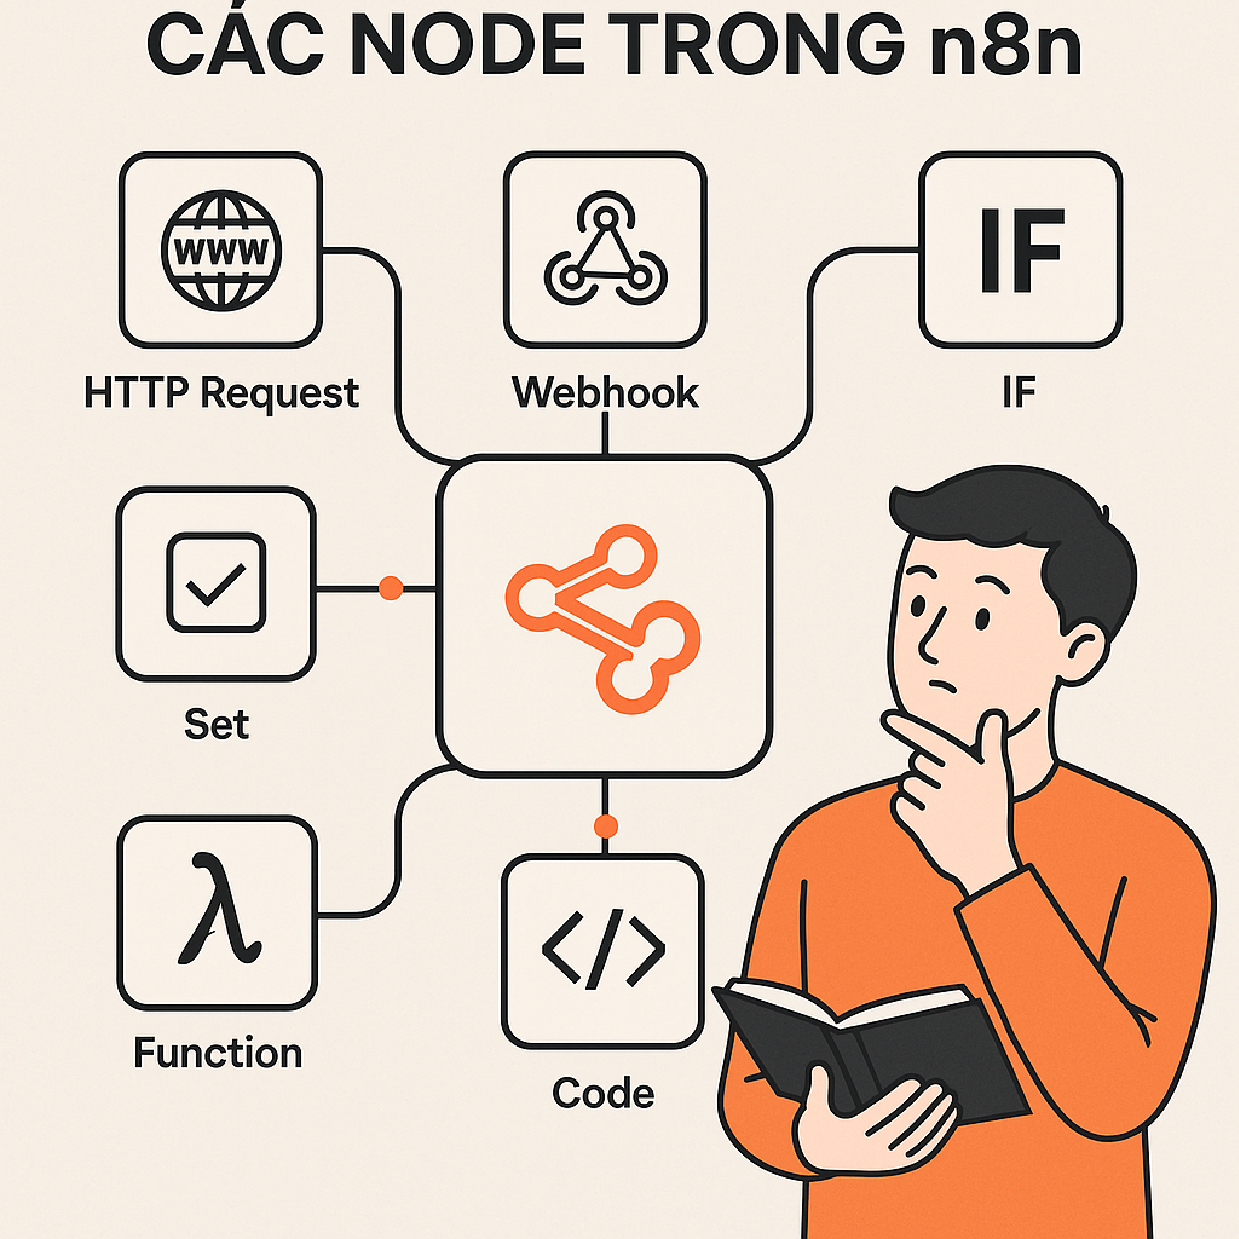
\includegraphics[width=0.96\linewidth]{Chap1-7/node-mh.pdf}
\end{figure}



Tưởng tượng này, bạn đang đứng giữa một công trường rộng lớn, nơi một ngôi nhà đang bắt đầu được dựng lên từ những viên gạch đầu tiên. Xung quanh bạn là tiếng búa, tiếng cưa, những thanh sắt đan xen vào nhau, và những người thợ đang cần mẫn làm việc. Lúc này, có thể bạn chưa thấy gì ngoài bê tông, thép, và bụi bặm – chưa có phòng khách ấm cúng, chưa có ánh đèn vàng hay chiếc ghế sofa yêu thích. Nhưng chính trong sự ngổn ngang ấy, nền móng của một tổ ấm đang dần hình thành.

Người chủ của ngôi nhà có thể đã tưởng tượng ra đủ điều – màu sơn tường, rèm cửa, cách bài trí từng góc nhỏ, thậm chí là cảm giác êm ái của đôi chân trần trên thảm phòng ngủ. Họ háo hức với những chi tiết hoàn mỹ, và có lẽ trong thâm tâm, họ mong có thể bỏ qua giai đoạn "lấm lem" của công trình, để bước thẳng vào phần thú vị nhất: trang trí và tận hưởng. Nhưng ai cũng hiểu rằng, nếu thiếu đi phần nền móng vững chắc, nếu không có những thanh xà ngang được liên kết chuẩn xác, thì chẳng có ngôi nhà nào đủ kiên cố để trường tồn. Những điều đẹp đẽ bên ngoài chỉ có thể toả sáng khi phần khung bên trong được xây dựng cẩn thận, tỉ mỉ.

Việc học lập trình, hay nói cụ thể hơn là học cách xây dựng quy trình tự động hoá trong n8n, cũng giống như vậy. Trong thế giới no-code, bạn không cần phải thông thạo những dòng code rối rắm hay hiểu sâu về các thuật toán phức tạp. Bạn không cần phải là một kỹ sư phần mềm lão luyện. Tuy nhiên, điều đó không có nghĩa là bạn có thể bỏ qua phần “nền móng”. Và trong n8n, các node chính là những viên gạch, là cột trụ, là hệ thống xương sống giúp mọi quy trình hoạt động trơn tru và hiệu quả.

Mỗi node trong n8n đóng vai trò như một công nhân trong đội xây dựng – có node chuyên kéo dữ liệu về, có node chịu trách nhiệm xử lý thông tin, có node phân nhánh điều kiện, và có node đảm nhận việc gửi kết quả đi. Khi bạn hiểu rõ vai trò và cách phối hợp giữa các node, bạn sẽ giống như một kiến trúc sư lành nghề, biết cách chọn vật liệu, sắp xếp không gian và tối ưu từng chi tiết nhỏ nhất. Ngược lại, nếu bạn chỉ kéo-thả mà không thật sự hiểu cách dữ liệu luân chuyển qua từng node, bạn đang xây một ngôi nhà chỉ để “đẹp bề ngoài” – và nó có thể đổ sụp bất cứ lúc nào khi quy trình phức tạp hơn, hoặc khi cần thay đổi điều gì đó.
\newpage

\section{Giao diện người dùng}

\begin{figure}[htbp]
    \centering
    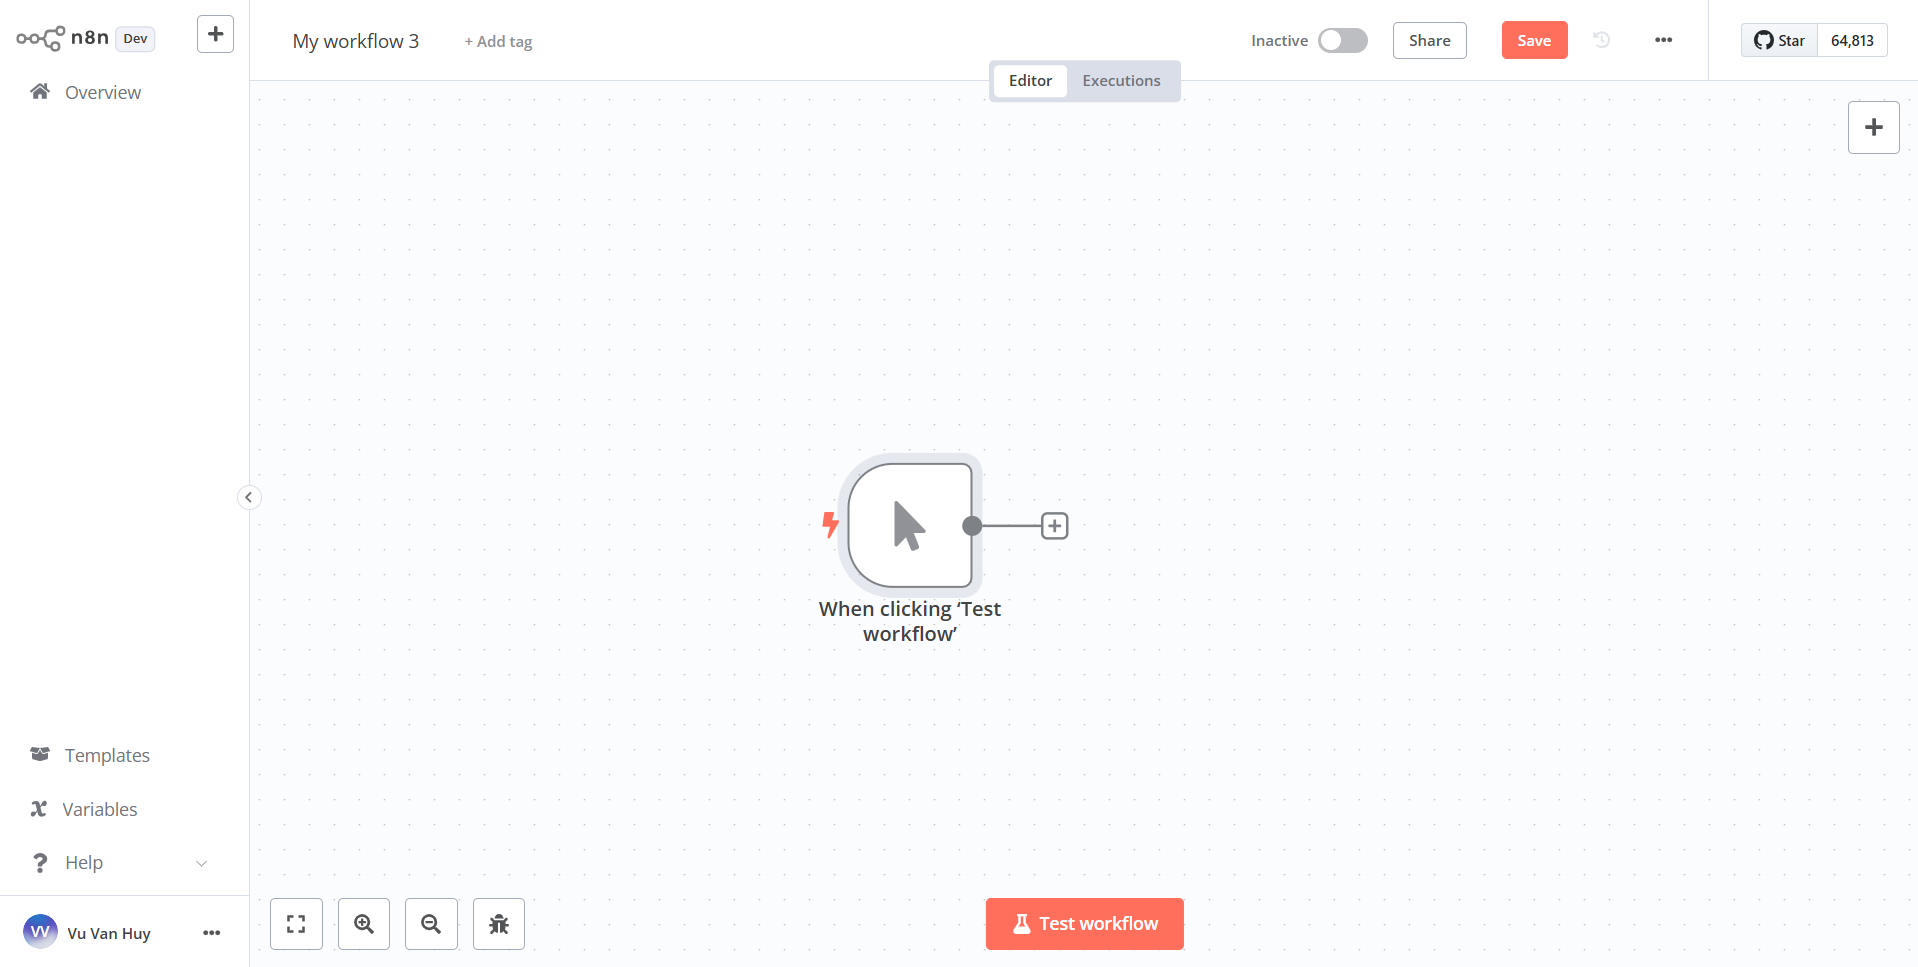
\includegraphics[width=1\linewidth]{Chap1-7/giaodien.png}
    \caption{Giao diện workflow ban đầu}
\end{figure}


Trong n8n, cấu trúc của một workflow bao gồm ba thành phần chính: Input, Output, và Trigger Node. Dưới đây là mô tả chi tiết về từng thành phần này:

\begin{itemize}
    \item Dashboard: Màn hình chính hiển thị danh sách các workflow, trạng thái của từng quy trình, log và các thông báo lỗi.
    \item Thanh Menu: Các mục điều hướng chính như  “Workflows”, “Executions”, “Credentials”, và “Settings”.
    \item Editor Workflow: Khu vực trung tâm dùng để kéo thả, sắp xếp và cấu hình các node.
\end{itemize}

    
Hướng dẫn điều hướng:
\begin{itemize}
    \item Thanh công cụ: Sử dụng các nút zoom, undo/redo và grid để dễ dàng quản lý các node trong workflow.
    \item Tìm kiếm và lọc: Hỗ trợ tìm kiếm workflow theo tên, trạng thái hay theo các từ khóa đã cấu hình.
\end{itemize}

\section{Ngôn ngữ của n8n}
Ngay từ nhỏ, tôi thích chu du khắp nơi, thích đi đây đi đó tìm kiếm những điều mới lạ về các sứ sở ngoài kia. Tôi rất thích và đam mê vẻ hào nhoáng của các đất nước nổi tiếng với nền văn hóa du lịch của họ. Bất lợi thay tôi ko thể trải nghiệm toàn bộ nền văn hóa này do tôi chỉ biết và sõi duy nhất một ngôn ngữ là tiếng mẹ đẻ. Việc này dẫn đến việc tôi thường xuyên hiểu sai nghĩa khi bất chợt tôi đọc một cái hay ho nào đó. 

n8n cũng có một ngôn ngữ riêng để các node giao tiếp với nhau. Ngôn ngữ này là JSON, một dạng key - value đơn giản dễ biên dịch cho cả người và máy, là một chuẩn để mô tả thông tin object phổ biến trong tất cả các phần mềm. Nhờ loại ngôn ngữ này chúng ta có thể dễ dàng truyền tải dữ liệu và văn bản dạng nhị phân. Các node đều có input và output dạng JSON. Chúng ta sẽ tìm hiểu kĩ loại ngôn ngữ này để dùng "Expression" để truy suất thông tin JSON  Vì vậy việc nắm vứng các sử dụng JSON là hết sức cần thiết. Và cuốn sách này sẽ nhắc tới rất nhiều ngôn ngữ này. 


\section{Node}

Trong n8n, nodes là các thành phần cơ bản và quan trọng nhất của mỗi workflow. Mỗi node đại diện cho một hành động, một dịch vụ, hoặc một chức năng cụ thể mà bạn muốn thực hiện. Có thể hình dung nodes như các khối xây dựng của quy trình tự động hóa của bạn.

\begin{figure}[htbp]
    \centering
    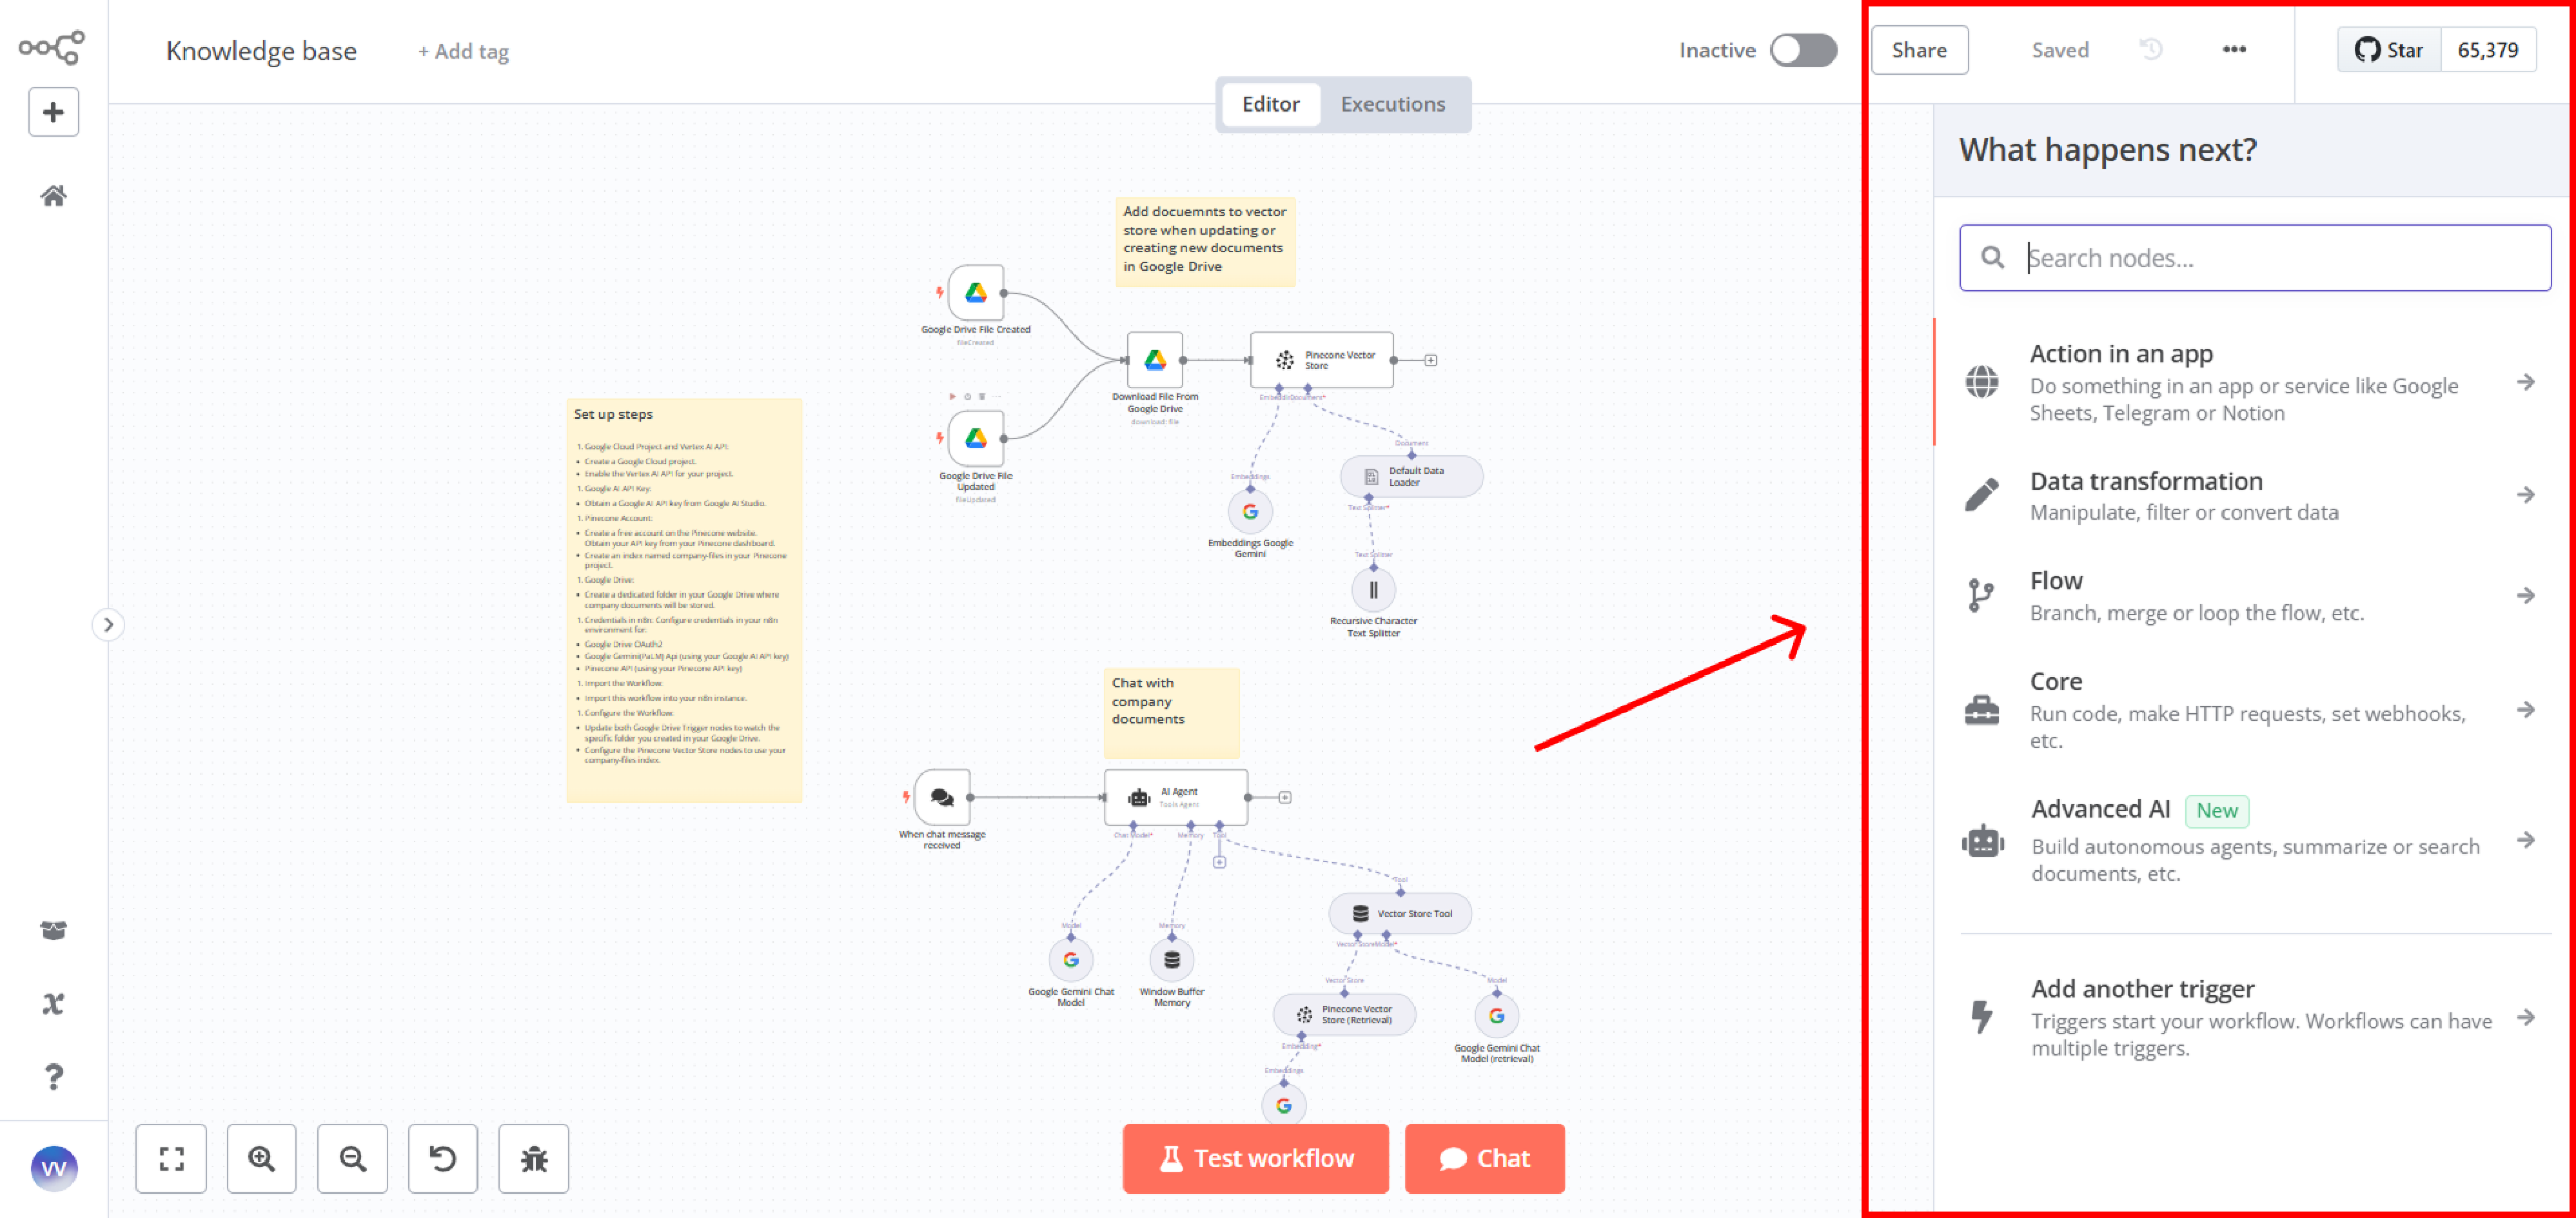
\includegraphics[width=1\linewidth]{Chap1-7/node.pdf}
    \caption{Các option chọn node}
\end{figure}

\newpage

\subsection{Chức năng chính của nodes}

\begin{figure}[htbp]
    \centering
    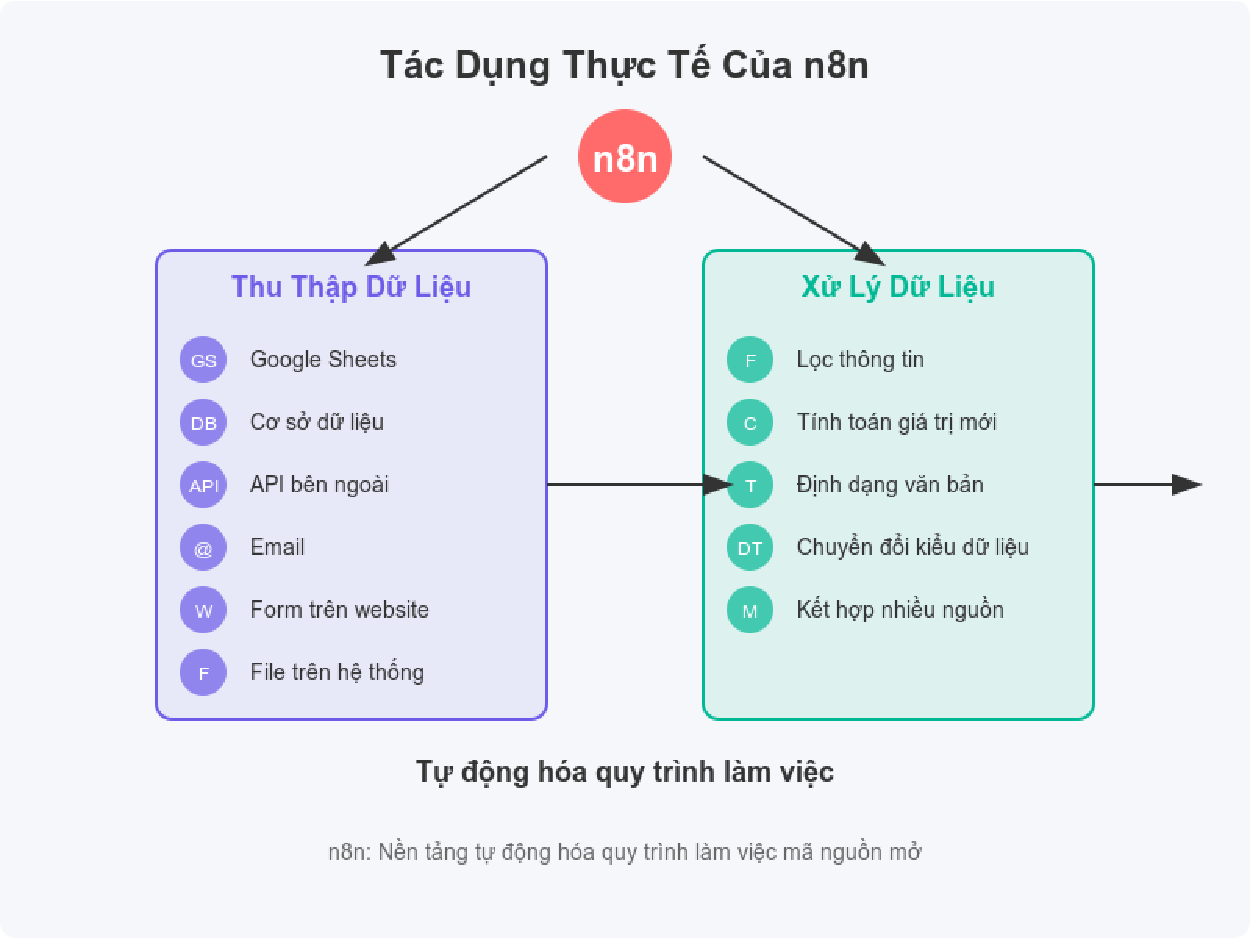
\includegraphics[width=1\linewidth]{Chap1-7/a.pdf}
    \caption{Tác dụng và chức năng thực tế của n8n}
\end{figure}

Các loại node cơ bản:
\begin{itemize}
    \item Trigger: Bắt đầu workflow (ví dụ: Webhook khi có dữ liệu).
    \item Action in app: Gọi tới một node khác không phải n8n (ví dụ: Gửi email).
\end{itemize}
Ví dụ: Nút Webhook giống như chuông cửa – khi có khách (dữ liệu), nó báo cho các nút khác hành động.

\newpage
\section{Cấu trúc của một node}


\subsection{Input}

\begin{figure}[htbp]
    \centering
    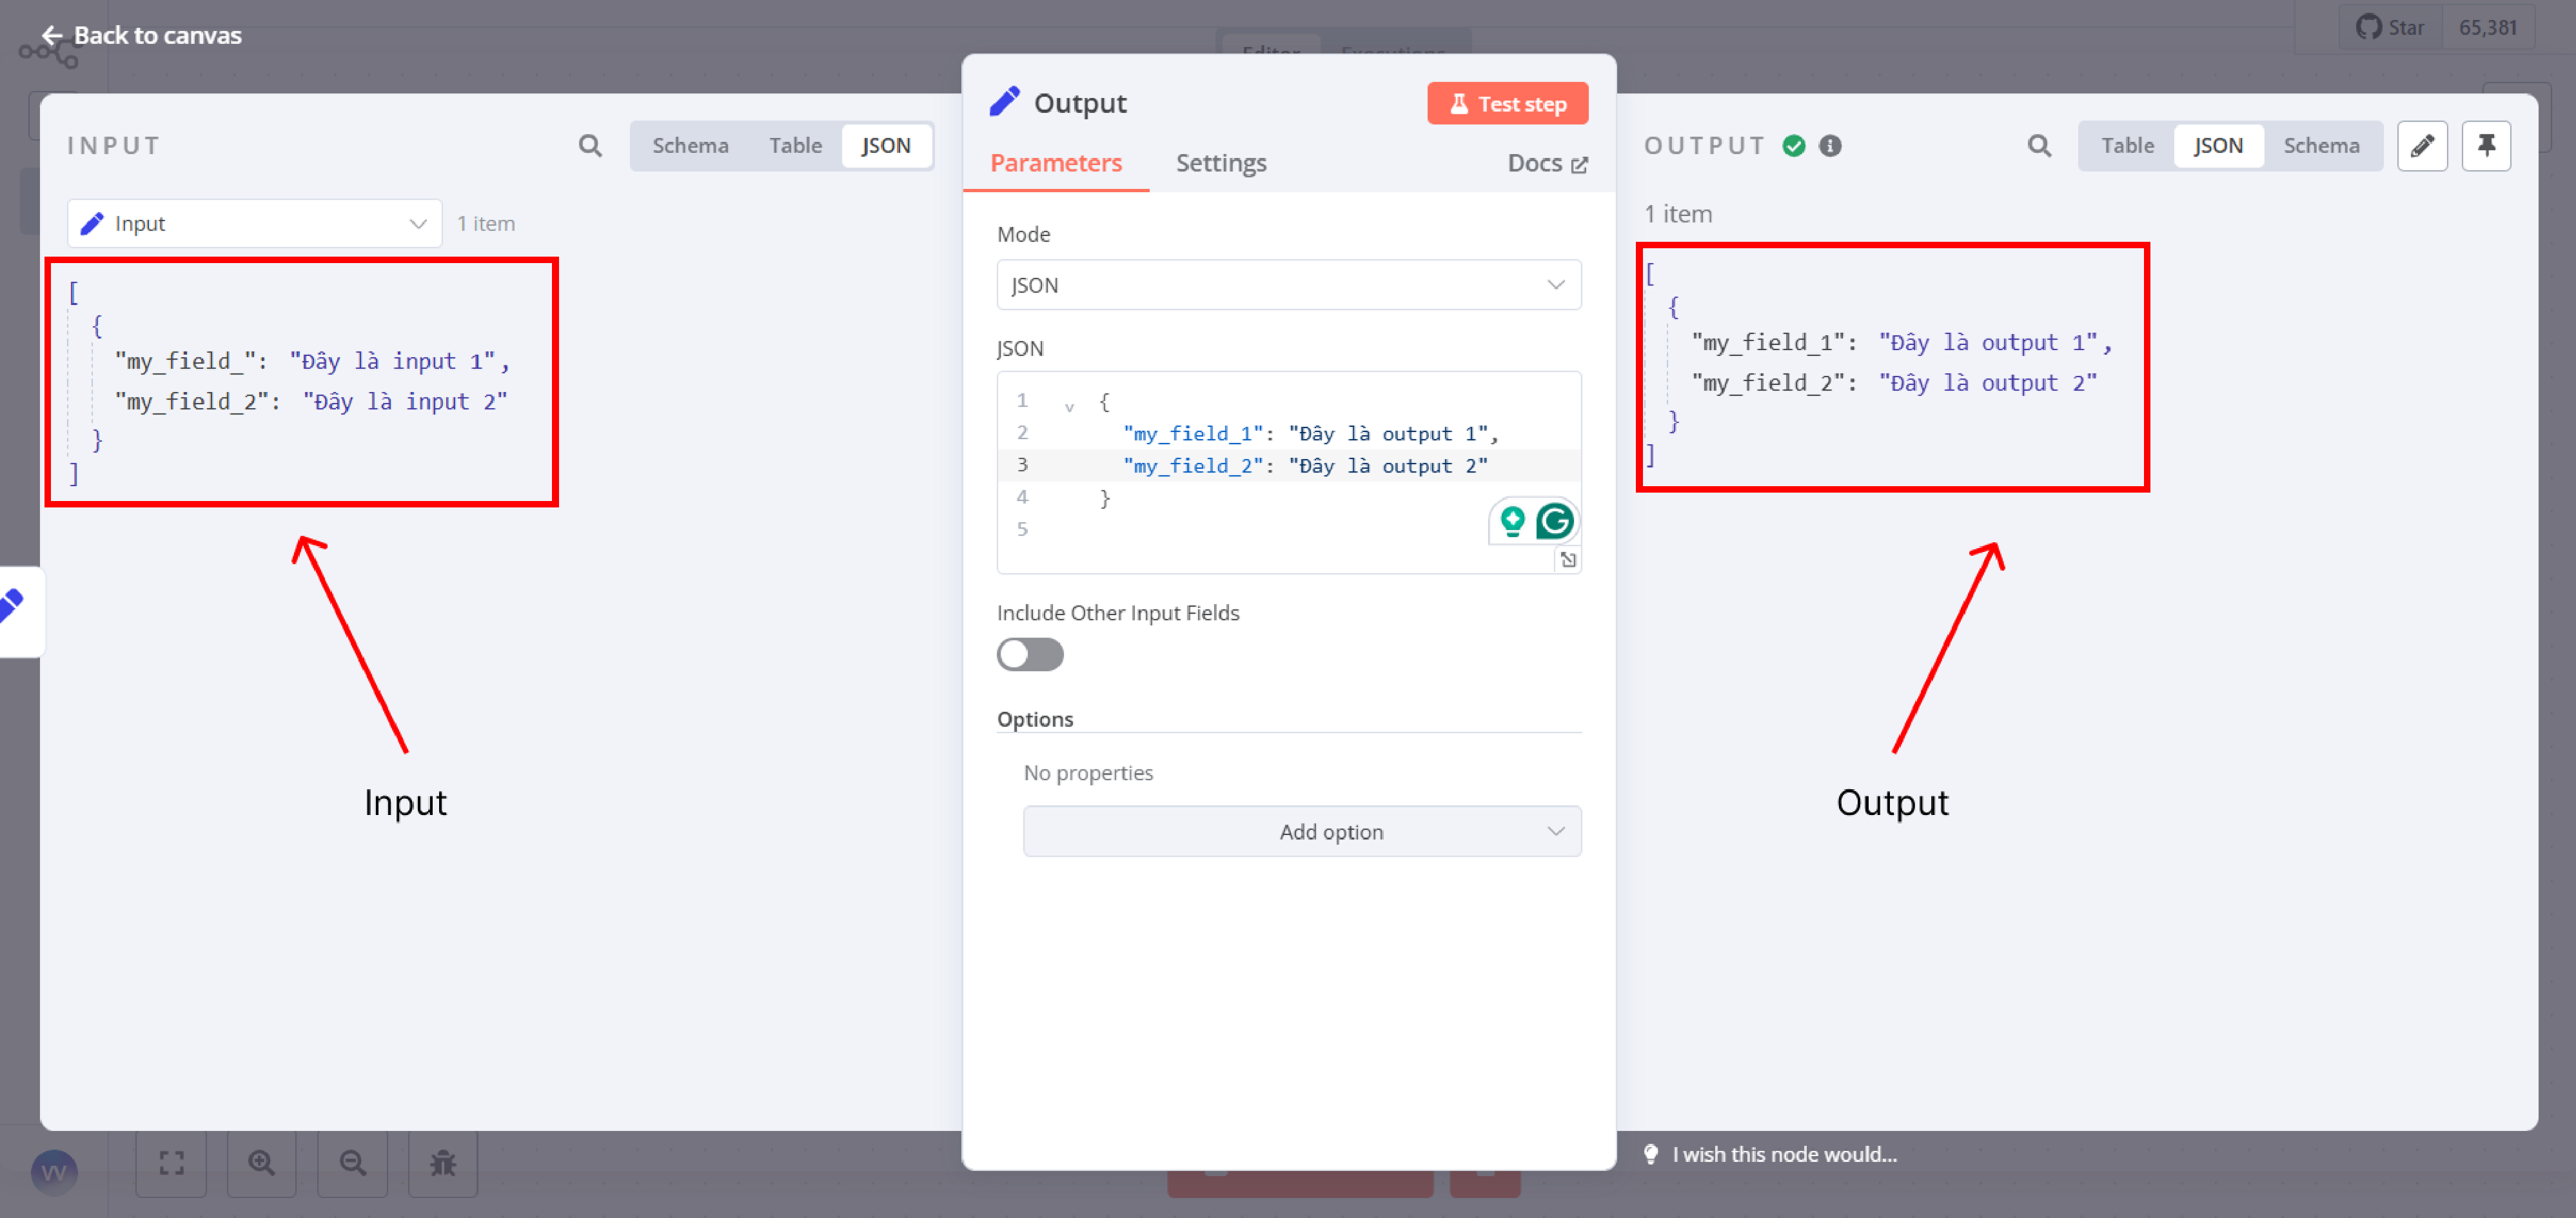
\includegraphics[width=1\linewidth]{Chap1-7/input-ouput.pdf}
\end{figure}

Input là dữ liệu mà node nhận được từ các node trước đó trong workflow. Mỗi node (trừ Trigger nodes) sẽ nhận dữ liệu đầu vào từ một hoặc nhiều node khác.

\begin{lstlisting}[language = Javascript]
{
  "items": [
    {
      "json": {
        "ten": "Nguyen Van A",
        "email": "nguyenvana@example.com",
        "tuoi": 30
      },
      "binary": {
        // Du lieu nhi phan nhu file, hinh anh
      }
    },
    {
      "json": {
        "ten": "Tran Thi B",
        "email": "tranthib@example.com",
        "tuoi": 25
      },
      "binary": {}
    }
  ]
}
\end{lstlisting}
Cấu trúc này có những đặc điểm quan trọng:
\begin{itemize}
    \item Items: Là một mảng các phần tử dữ liệu, mỗi phần tử là một bản ghi riêng biệt
    \item json: Chứa dữ liệu dạng JSON của mỗi item
    \item binary: Chứa dữ liệu nhị phân như file, hình ảnh
\end{itemize}

Khi một node xử lý xong và chuyển dữ liệu sang node tiếp theo, dữ liệu vẫn duy trì cấu trúc này.

\clearpage
\subsection{Parameters}
Parameters là các cài đặt và tùy chọn mà bạn có thể thiết lập cho mỗi node. Chúng quyết định cách node hoạt động và xử lý dữ liệu.

Các loại parameters phổ biến:

\begin{figure}[htbp]
    \centering
    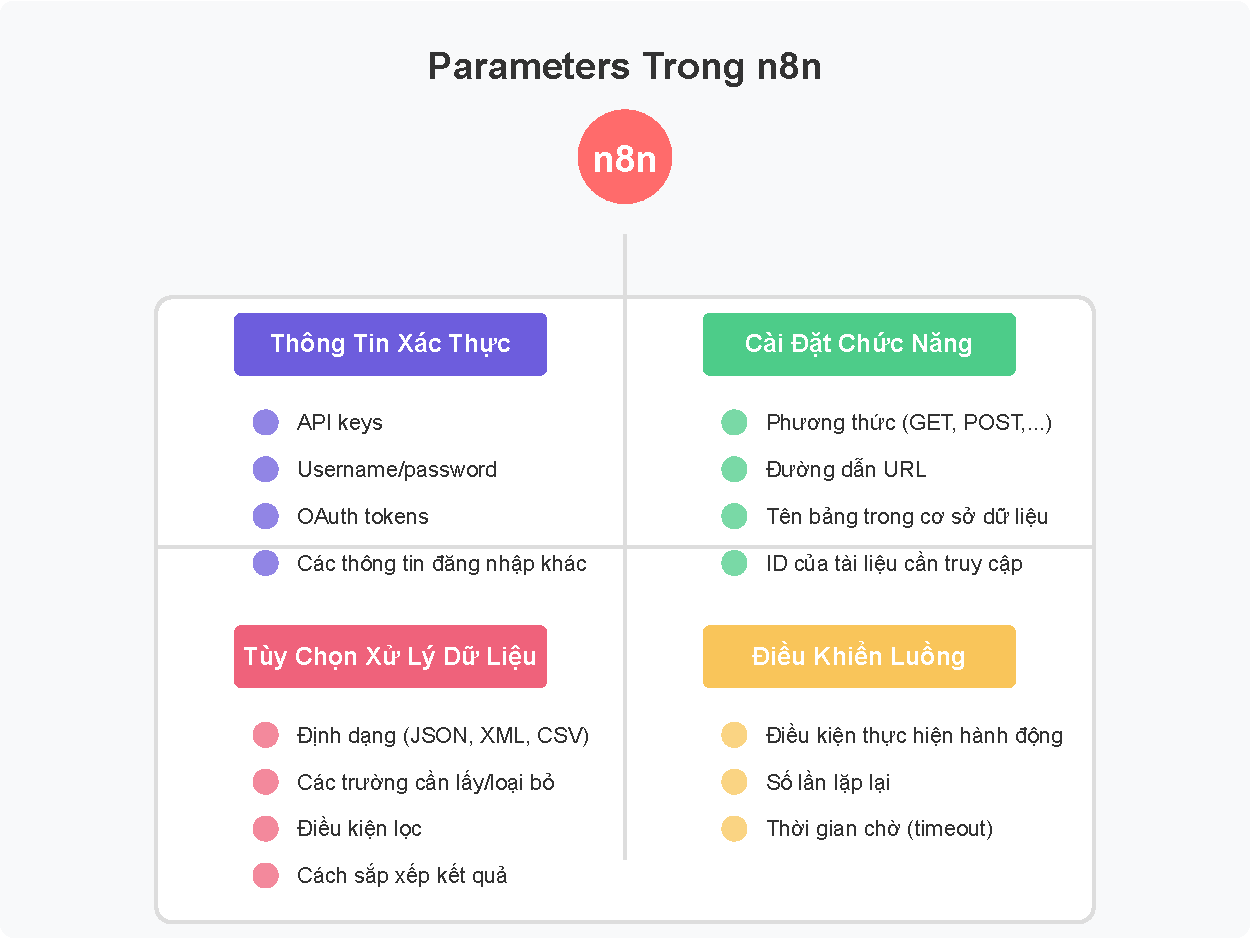
\includegraphics[width=1\linewidth]{Chap1-7/parameters.pdf}
    % \caption{Caption}
\end{figure}

Ví dụ về parameters trong HTTP Request node:
\begin{lstlisting}   
Method: POST
URL: https://api.example.com/users
Headers:
  Content-Type: application/json
  Authorization: Bearer abc123xyz
Query Parameters:
  limit: 10
  offset: 0
Request Body:
  {
    "name": "Nguyen Van A",
    "email": "nguyenvana@example.com"
  }
\end{lstlisting}


\subsection{Output}
Output là kết quả sau khi node thực hiện xong công việc của nó. Output này sẽ trở thành input cho node tiếp theo trong workflow.
Output tuân theo cùng cấu trúc với input:
\begin{itemize}
    \item Mảng các items
    \item Mỗi item có phần json và binary
\end{itemize}

Ví dụ output từ HTTP Request node lấy danh sách người dùng:

\begin{lstlisting}[language = Javascript]   
{
  "items": [
    {
      "json": {
        "id": 1,
        "name": "Nguyen Van A",
        "email": "nguyenvana@example.com",
        "createdAt": "2023-01-15T08:30:00Z"
      }
    },
    {
      "json": {
        "id": 2,
        "name": "Tran Thi B",
        "email": "tranthib@example.com",
        "createdAt": "2023-02-20T10:45:00Z"
      }
    }
  ]
}
\end{lstlisting}


\subsection{Kết nối các nút để tạo luồng dữ liệu}

\begin{figure}[htbp]
    \centering
    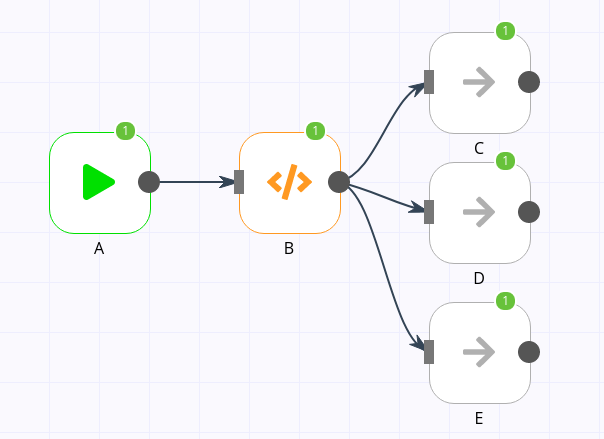
\includegraphics[width=0.6\linewidth]{Chap1-7/node.png}
    \caption{Minh họa node trong n8n}
\end{figure}


\begin{itemize}
    \item Kéo dây từ chấm tròn "Output" của nút này sang chấm tròn "Input" của nút khác.
    \item Dữ liệu sẽ chảy qua dây nối đó.
\end{itemize}

Ví dụ: Nối Webhook với Gmail để dữ liệu từ Webhook được gửi qua email.

\section{Trigger Node}
Trigger nodes là điểm khởi đầu của mọi workflow. Chúng xác định khi nào workflow sẽ được kích hoạt và thực thi. Một workflow luôn bắt đầu bằng ít nhất một trigger node.

\begin{enumerate}
    \item Webhook Node

Webhook node kích hoạt workflow khi nhận được một HTTP request từ bên ngoài.

Ví dụ cấu hình:
\begin{lstlisting}
Method: POST
Path: /new-order
Authentication: username/password
\end{lstlisting}

\textbf{Ứng dụng thực tế:}
\begin{itemize}
    \item Nhận thông báo khi có đơn hàng mới từ website
    \item Tích hợp với dịch vụ thanh toán như PayPal, Stripe
    \item Nhận dữ liệu từ IoT devices
\end{itemize}

\item Cron Node

Cron node kích hoạt workflow theo lịch trình định kỳ, sử dụng cú pháp cron.

Ví dụ cấu hình:
% Làm thế nào đấy để đóng khung cái này vào
\begin{itemize}
    \item 0 9 * * 1-5    (Chạy lúc 9 giờ sáng mỗi ngày từ thứ 2 đến thứ 6)
    \item 0 */2 * * *    (Chạy mỗi 2 giờ)
    \item 0 0 1 * *      (Chạy vào 0 giờ ngày 1 hàng tháng)
\end{itemize}

\textbf{Ứng dụng thực tế:}
\begin{itemize}
    \item Tạo báo cáo hàng ngày/tuần/tháng
    \item Sao lưu dữ liệu định kỳ
    \item Gửi email nhắc nhở
\end{itemize}

\item Email Trigger Node

Email Trigger node kích hoạt workflow khi nhận được email mới phù hợp với tiêu chí đã đặt.

Ví dụ cấu hình:
\begin{itemize}
    \item Email account: support@example.com
    \item Folder: INBOX
    \item Include: Subject contains "urgent"
\end{itemize}

\textbf{Ứng dụng thực tế:}
\begin{itemize}
    \item Tự động phản hồi email
    \item Tạo ticket hỗ trợ từ email
    \item Lưu trữ tệp đính kèm
\end{itemize}

\item Form Trigger Node

Form Trigger node tạo một form online và kích hoạt workflow khi form được submit.

% Ví dụ cấu hình:

% Fields:

% - Name (text)

% - Email (email)

% - Message (textarea)

% - Priority (dropdown: Low, Medium, High)

% Ứng dụng thực tế:

% \begin{itemize}
%     \item Thu thập phản hồi khách hàng
%     \item Đăng ký sự kiện
%     \item Tạo lead từ website
% \end{itemize}

\end{enumerate}

\newpage
\section{Data transformation}

\subsection{Node Set}
\begin{figure}[htbp]
    \centering
    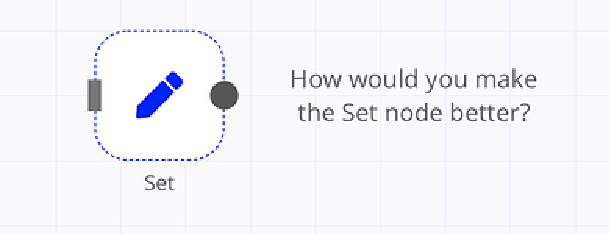
\includegraphics[width=0.8\linewidth]{Chap1-7/set-node.pdf}
\end{figure}

Node này là node rất hay sử dụng. Thường thì mọi người hay cho mình template và sử dụng node set này để thiết lập một số thông tin trong quá trình workflow chạy chúng ta có thể sử dụng node set này để tạo ra các biến mới giúp thông tin gọn gàng hơn

Đây là một node khá đơn giản


1 số cấu hình: "Inputed Fields to include" -> Chọn Selected -> Chỉ chọn biến còn lại bỏ, lấy từ node set trước -> Giúp gọn gàng hơn


\subsection{Split out}

\begin{figure}[htbp]
    \centering
    
\includegraphics[width=0.4\linewidth]{Chap1-7/split-out.pdf}
\end{figure}

Giả sử bạn có đoạn json như này, bạn ko có kiến thức về code hay lập trình. Và bạn vẫn muốn cắt đoạn json này thành các bản ghi tương ứng theo dòng và theo đối tượng. Thì node Split out là lựa chọn phù hợp cho bạn.

\begin{verbatim}
{
  "payments": [
    {
      "transactionId": "TXN1001",
      "payerName": "Nguyễn Hoàng Long",
      "amount": 1500000,
      "method": "Chuyển khoản",
      "date": "2025-04-05",
      "status": "Thành công"
    },
    {
      "transactionId": "TXN1002",
      "payerName": "Trần Thu Hà",
      "amount": 850000,
      "method": "Thẻ tín dụng",
      "date": "2025-04-04",
      "status": "Đang xử lý"
    },
    {
      "transactionId": "TXN1003",
      "payerName": "Lê Văn Hùng",
      "amount": 420000,
      "method": "Tiền mặt",
      "date": "2025-04-03",
      "status": "Thất bại"
    }
  ]
}
\end{verbatim}

Split out sẽ lấy các thuộc tính bên trong ra 

\newpage

Kết quả nhận được:

\begin{figure}[htbp]
    \centering
    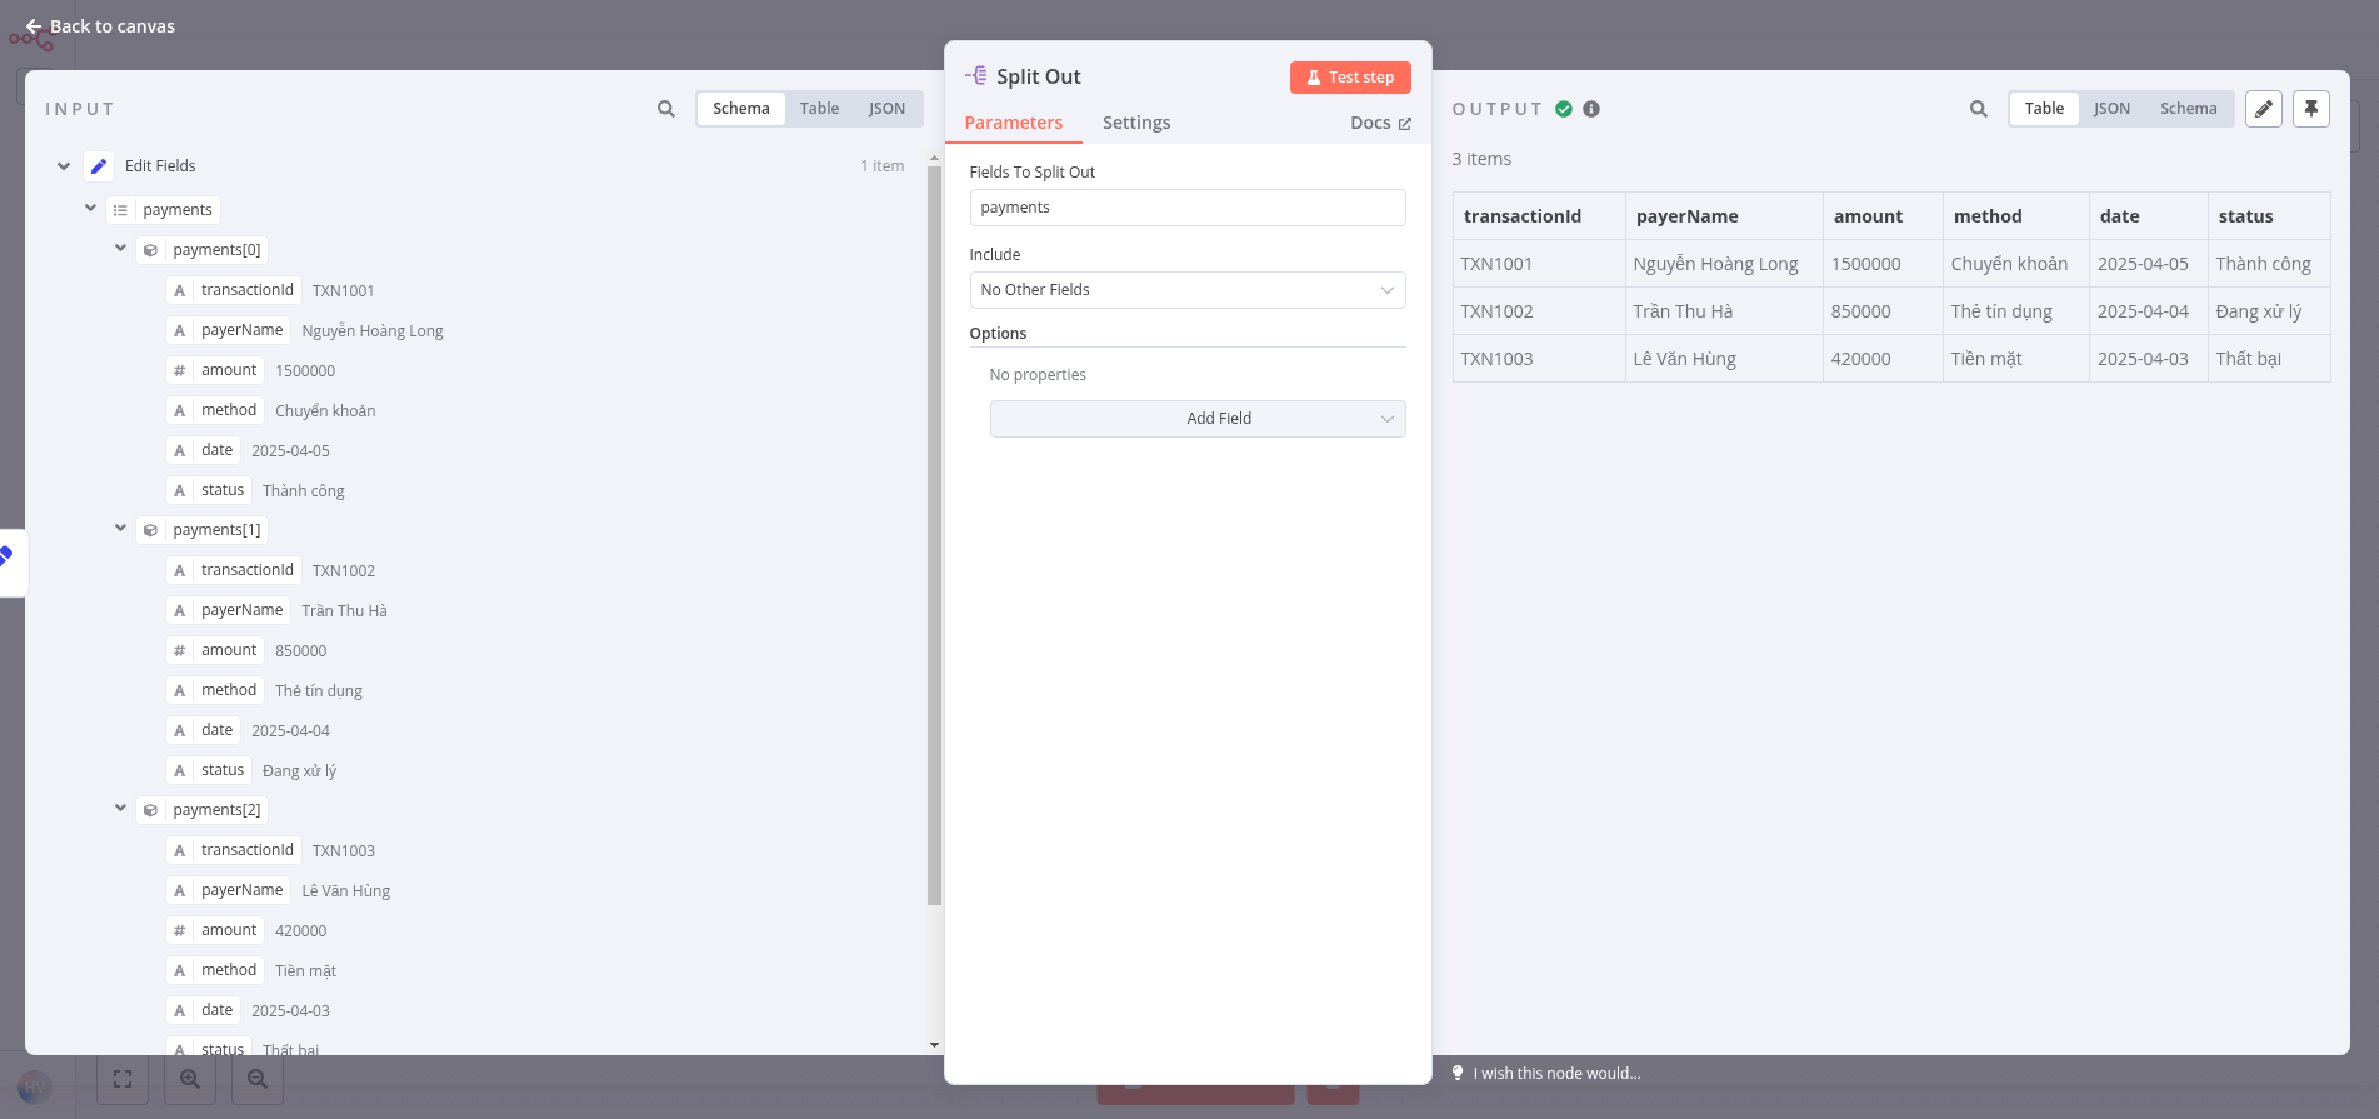
\includegraphics[width=1\linewidth]{Chap1-7/splitout.pdf}
\end{figure}

$\Rightarrow$ Đại khái hiểu cái này như unest trong sql.

\subsection{Node merge}
\begin{figure}[htbp]
    \centering
    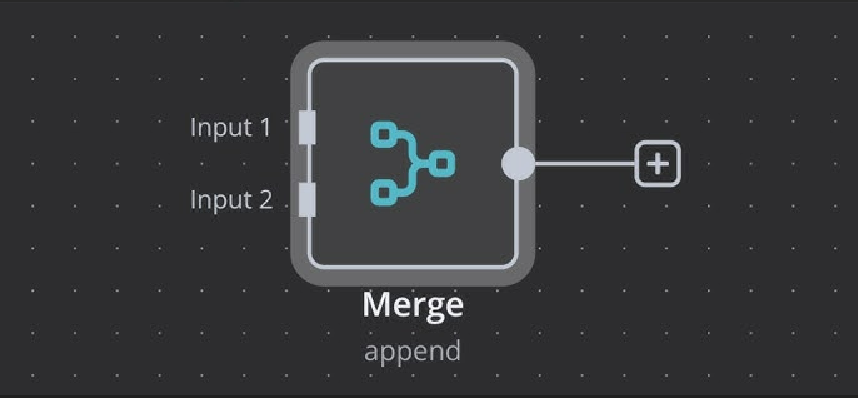
\includegraphics[width=0.8\textwidth]{Chap1-7/merge-merge.pdf}
\end{figure}

Node Merge trong n8n cho phép bạn kết hợp dữ liệu đầu ra từ nhiều node khác nhau thành một luồng dữ liệu duy nhất. Điều này đặc biệt hữu ích khi bạn cần tổng hợp thông tin từ các nguồn khác nhau hoặc khi bạn có các nhánh xử lý song song cần được hợp nhất.

Có nhiều chế độ:

\begin{itemize}
    \item Append
    \item Merge by Fields
    \item Merge by Position
    \item Pass-throught
\end{itemize}
1. Append: Thêm vào

Mô tả: Thêm tất cả các mục từ tất cả các đầu vào thành một mảng duy nhất. Sử dụng khi muốn tập hợp tất cả các dữ liệu từ nhiều nguồn mà không cần quan tâm đến việc ghép nối chúng với nhau

2. Merge By Fields: Hợp nhất theo trường

Mô tả: Kết hợp các mục dựa trên các trường khóa được chỉ định
Trường hợp sử dụng: Khi các mục từ các nguồn khác nhau liên quan đến nhau thông qua một trường chung

3. Merge By Position: Hợp nhất theo vị trí

Mô tả: Kết hợp các mục dựa trên vị trí của chúng trong mảng
Trường hợp sử dụng: Khi thứ tự của dữ liệu đầu vào tương ứng với nhau

4. Pass-through: Truyền qua

Mô tả: Truyền qua tất cả các mục từ một đầu vào cụ thể
Trường hợp sử dụng: Khi bạn cần ưu tiên một luồng dữ liệu nhưng vẫn muốn đợi cho đến khi tất cả các kết nối đầu vào đã xử lý xong

$\Rightarrow$ Phần này là intro thôi, phần sau sẽ kĩ hơn.


Ngoài ra còn cái node khác:


- edit filed

- Remove duplicate

- filter

- limit

- Edit image

- Markdown

- Convert

- Extract from file

- HTML


- Crypto

\section{Flow node}

Flow control nodes cho phép bạn kiểm soát cách dữ liệu di chuyển qua workflow, tạo các nhánh rẽ và kết hợp dữ liệu.
\begin{enumerate}
    \item \textbf{IF Node}  
    IF node tạo hai nhánh dựa trên một điều kiện: true (đúng) và false (sai).  

    Ví dụ cấu hình:
\begin{lstlisting}[language=JavaScript]
Condition: {{ $input.item.json.amount > 1000000 }}    
\end{lstlisting}

    Với cấu hình này:
    \begin{itemize}
        \item Nếu giá trị \texttt{amount} lớn hơn 1,000,000, dữ liệu sẽ đi theo nhánh \textbf{TRUE}.
        \item Nếu giá trị \texttt{amount} nhỏ hơn hoặc bằng 1,000,000, dữ liệu sẽ đi theo nhánh \textbf{FALSE}.
    \end{itemize}
    
    \item \textbf{Switch Node}  
    Switch node tạo nhiều nhánh dựa trên giá trị của một trường.  

    Ví dụ cấu hình:
\begin{lstlisting}[language=JavaScript]
Field: {{ $input.item.json.status }}
Case 1: "new" -> Output 1
Case 2: "processing" -> Output 2
Case 3: "completed" -> Output 3
Case 4: "cancelled" -> Output 4
Default: Output 5 (other value)
\end{lstlisting}

    Ứng dụng:
    \begin{itemize}
        \item Định tuyến ticket hỗ trợ dựa trên phòng ban.
        \item Xử lý đơn hàng dựa trên trạng thái.
        \item Phân loại email dựa trên chủ đề.
    \end{itemize}

    \item \textbf{Merge Node}  
    Merge node kết hợp dữ liệu từ nhiều nhánh khác nhau trong workflow.  

    Ví dụ cấu hình:
\begin{verbatim}
Mode: Merge By Position
    - Ghep du lieu theo vi tri (item 1 tu input 1 + item 1 tu input 2)
    
    or
    
Mode: Merge By Fields
    - Truong de ghep: "id"
    - Ghep cac items co cung gia tri id tu cac input khac nhau
\end{verbatim}

    Ứng dụng:
    \begin{itemize}
        \item Kết hợp thông tin khách hàng từ nhiều nguồn.
        \item Ghép dữ liệu đơn hàng với thông tin vận chuyển.
        \item Tạo báo cáo tổng hợp từ nhiều bộ dữ liệu.
    \end{itemize}

    \item \textbf{Split In Batches Node}  
    Split In Batches node chia một tập dữ liệu lớn thành các nhóm nhỏ hơn để xử lý.  

    Ví dụ cấu hình:
\begin{verbatim}
Batch Size: 10
    - Chia du lieu thanh cac nhom, moi nhom 10 items
    - Moi nhom se duoc xu ly tuan tu
\end{verbatim}


    Ứng dụng:
    \begin{itemize}
        \item Xử lý hàng loạt email marketing.
        \item Gửi dữ liệu lớn đến API có giới hạn số lượng request.
        \item Tối ưu hóa hiệu suất khi xử lý dữ liệu lớn.
    \end{itemize}
\end{enumerate}

\subsection{Wait}
Dừng workflow tạm thời tại một điểm nhất định – cho đến khi:
\begin{enumerate}
    \item Một khoảng thời gian trôi qua (Time Duration), hoặc
    \item Đến một thời điểm cụ thể (Specific Date \& Time), hoặc

    \item Khi có tín hiệu từ node Webhook hoặc Wait → Resume (External Resume).
\end{enumerate}

Node này cực kỳ hữu ích khi bạn:
\begin{enumerate}
    \item Gửi email rồi đợi vài giờ mới kiểm tra phản hồi.

    \item Đợi một sự kiện từ người dùng (qua webhook).

    \item Chờ đến một thời điểm cụ thể (ví dụ: đến 9h sáng hôm sau mới gửi báo cáo
\end{enumerate}

\subsection{Kết nối giữa các Nodes}

Các nodes trong n8n được kết nối với nhau để tạo ra luồng dữ liệu. Dữ liệu sẽ di chuyển từ trigger node đến input nodes, sau đó qua các bước xử lý và cuối cùng đến output nodes. Việc kết nối này giúp đảm bảo rằng dữ liệu được truyền tải một cách mạch lạc và tự động hóa quy trình làm việc hiệu quả hơn.

$\Rightarrow$Tóm lại, cấu trúc của một workflow trong n8n bao gồm Trigger Node để khởi động quy trình, Input Nodes để thu thập dữ liệu đầu vào, và Output Nodes để thực hiện các hành động dựa trên dữ liệu đó.


\subsection{Mẹo sử dụng Node hiệu quả}

\begin{itemize}
    \item Đặt tên rõ ràng: Gọi node là "Gửi Email Nhắc Nhở" thay vì để mặc định "Email1" để dễ theo dõi.
    \item Kiểm tra từng bước: Dùng nút "Execute Node" để kiểm tra từng node trước khi chạy toàn bộ workflow.
    \item Tận dụng dữ liệu giữa các Node: Dữ liệu từ node trước (như thời gian từ Cron) có thể được dùng ở node sau (như thêm thời gian vào email).
\end{itemize}


\section{Core node}

\subsection{HTTP request}
Trước khi đi sâu vào Node HTTP Request hãy chậm lại để hiểu về API đã. Web API hoạt động dựa trên cùng nền tảng công nghệ quen thuộc với hầu hết các trang web bạn lướt qua hàng ngày trên internet. Nhưng thay vì mang đến những trang web yêu thích hay những đoạn video mèo con đáng yêu, các máy chủ web được thiết lập để vận hành API mở ra cánh cửa cho các hệ thống từ xa gửi yêu cầu và nhận về dữ liệu phản hồi dựa trên thông tin đầu vào. Dữ liệu luân chuyển giữa các hệ thống này thường được gói gọn trong định dạng JSON – gọn gàng và đầy sức mạnh!

Để chứng kiến một API cơ bản hoạt động, hãy thử nghiệm với Random User API. Mở trình duyệt của bạn và nhập vào thanh địa chỉ: https://randomuser.me/api/. Thoạt nhìn, bạn có thể thấy một chuỗi ký tự khó hiểu, nhưng nếu quan sát kỹ, bạn sẽ nhận ra một vài điểm tương đồng với những gì chúng ta đã học ở chương về node Function. Thứ bạn đang thấy chính là JSON ở dạng nén hoặc chưa được định dạng đẹp mắt!

Để truy cập được API, một thứ item thiết yếu phải cần là URL. Việc hiểu rõ và thiết kế API vô cùng quan trọng vì bạn luôn muốn điều chỉnh đầu ra để đạt được kết quả mong muốn. 


Thử quan sát một API và phân tích nó:

\begin{verbatim}
https://api.example.com/v3/computers?type=laptop&ram=32&hdd=1024
\end{verbatim}

Các thành phần của một URL API

\begin{enumerate}
    \item Giao thức (Protocol)

Trong ví dụ trên, phần https:// chính là giao thức.

Thông thường, giao thức sẽ là http:// hoặc https://.

Điều quan trọng cần nhớ là nếu dùng http://, dữ liệu sẽ không được mã hóa giữa máy khách và máy chủ API, có thể dẫn đến rủi ro bảo mật.

Vì vậy, luôn đảm bảo sử dụng https:// để đảm bảo an toàn cho dữ liệu.

    \item Base URL

Trong ví dụ, api.example.com chính là base URL, đôi khi còn được gọi là hostname, domain name hoặc DNS name.
Đây là địa chỉ máy chủ nơi API được lưu trữ.

    \item Endpoint
    
Endpoint trong URL trên là /v3/computers, đôi khi được gọi là API path.
Endpoint có thể là tĩnh (không thay đổi) hoặc động (thay đổi dựa trên dữ liệu được yêu cầu).

Ví dụ trên có hai phần:

/v3 → Cho biết đây là phiên bản thứ 3 của API.

/computers → Chỉ ra rằng API này sẽ trả về thông tin về một hoặc nhiều máy tính.

    \item  Query Parameters
    

\tcbset{colback=red!5!white,colframe=red!75!black}
\begin{tcolorbox}[title=Các tham số truy vấn trong ví dụ là:]
\begin{itemize}
    \item type=laptop

    \item ram=32

    \item hdd=1024
\end{itemize}
\end{tcolorbox}


\tcbset{colback=red!5!white,colframe=red!75!black}
\begin{tcolorbox}[title=Chúng được xác định bởi hai dấu phân cách:]
\begin{itemize}
    \item Dấu ? → Tách các tham số truy vấn khỏi phần còn lại của URL.

    \item Dấu \& → Ngăn cách từng tham số truy vấn.

    \item Tương tự như trong JSON, mỗi tham số có dạng cặp key-value:
    \begin{itemize}
        \item key → Phần trước dấu =.

       \item value → Phần sau dấu =.
    \end{itemize}

\end{itemize}
\end{tcolorbox}


Các thành phần khác trong API Request
\begin{enumerate}
    \item Headers



\tcbset{colback=orange!5!white,colframe=orange!75!black}
\begin{tcolorbox}[title=Headers chứa metadata về request API chẳng hạn như:]
\begin{itemize}
    \item Loại dữ liệu truyền tải.

    \item Token xác thực.

    \item Thông tin về máy chủ.

    \item Headers thường có định dạng key-value.
\end{itemize}
\end{tcolorbox}



    \item Body Parameters
Body chứa dữ liệu được gửi kèm trong request, thường có dạng key-value.

Các phương thức HTTP (HTTP Methods)
Các phương thức HTTP là cách để API xử lý request từ client.


\tcbset{colback=green!5!white,colframe=green!75!black}
\begin{tcolorbox}[title=Dưới đây là một số phương thức phổ biến:]
\begin{itemize}
    \item GET → Lấy dữ liệu từ API (tương tự khi truy cập một trang web).

    \item POST → Gửi dữ liệu mới đến API để lưu trữ.

    \item DELETE → Xóa một tài nguyên hoặc bản ghi trên máy chủ API.

    \item HEAD → Giống GET nhưng chỉ trả về phần header, không có dữ liệu.

    \item PATCH → Cập nhật một phần thông tin trong bản ghi hiện có.

    \item PUT → Nếu bản ghi đã tồn tại, ghi đè dữ liệu cũ bằng dữ liệu mới; nếu chưa có, tạo bản ghi mới.
\end{itemize}
\end{tcolorbox}




Khi gửi request đến API, máy chủ sẽ trả về một mã phản hồi để báo trạng thái của request:

\tcbset{colback=green!5!white,colframe=green!75!black}
\begin{tcolorbox}[title=Mã phản hồi HTTP (Response Codes)]
\begin{itemize}
    \item 1xx (Thông tin) → Máy chủ đã nhận request và đang xử lý.

    \item 2xx (Thành công) → Request đã được xử lý thành công.

    \item 3xx (Chuyển hướng) → API đã được di chuyển đến một địa chỉ khác.

    \item 4xx (Lỗi từ phía client) → Request bị sai, cần kiểm tra và chỉnh sửa.

    \item 5xx (Lỗi từ phía server) → Máy chủ API có vấn đề, không thể xử lý request.
\end{itemize}
\end{tcolorbox}





Bây giờ, khi đã hiểu rõ về API URL, chúng ta sẽ bắt đầu sử dụng HTTP Request node trong n8n để kết nối với API! 
\end{enumerate}

\end{enumerate}



\subsection{Code}

Bạn nghĩ rằng n8n là công cụ nocode và bạn sẽ có node phù hợp cho workflow của bạn. Thật không may không có node nào là đa năng cả. Điều này hoàn toàn dễ hiểu do trong thực tế có vô vàn điều có thể xảy ra. 

$\Rightarrow$ Vì vậy n8n tạo ra Function Code cho phép thực thi mã Javascript để xử lý các trường hợp khó bằng code. 

Không giống như nhiều node khác có sẵn các tùy chọn và tham số để lựa chọn, Function node chỉ có duy nhất một tham số—trường nhập mã JavaScript. Toàn bộ thao tác xử lý dữ liệu của bạn sẽ được thực hiện trong trường này.

Trong JavaScript code field, bạn sẽ viết mã JavaScript để thao tác dữ liệu bên trong Function node.
Mặc dù bạn không cần phải là một chuyên gia về JavaScript, nhưng việc hiểu cơ bản về ngôn ngữ này sẽ mang lại nhiều lợi ích. Đối với nội dung trong cuốn sách này, chỉ cần nắm vững những kiến thức JavaScript cơ bản là đủ.


\subsection{Webhook}
Node Webhook hoạt động như một "người nghe" - khi có sự kiện xảy ra, webhook sẽ nhận thông báo và kích hoạt hành động tương ứng.

\textbf{Tính năng chính:}

\begin{itemize}
    \item Hỗ trợ các phương thức HTTP: GET, POST, PUT, DELETE
    \item Xác thực với Basic Auth hoặc Header Auth  
    \item Tự động phân tích dữ liệu JSON, form data và query parameters
    \item Có thể tạo phản hồi tùy chỉnh cho người gửi request
\end{itemize}

Ví dụ: Bot thông báo thời tiết đơn giản:

\begin{enumerate}
    \item Tạo một node Webhook với phương thức POST ở path \texttt{/weather}
    \item Khi có request gửi đến với dữ liệu: \texttt{\{"city": "Hanoi"\}}
    \item Sử dụng HTTP Request node để gọi API thời tiết với thành phố từ request
    \item Định dạng kết quả và gửi thông báo thời tiết qua Telegram
    \item Trả về phản hồi thành công cho request ban đầu
\end{enumerate}

\textbf{Gọi webhook}
\begin{lstlisting}
curl -X POST https://n8n.yourdomain.com/webhook/weather \
  -H "Content-Type: application/json" \
  -d '{"city": "Hanoi"}'
\end{lstlisting}

Người dùng sẽ nhận được thông báo: \textit{"Thời tiết tại Hanoi hiện tại là 28°C, trời quang. Độ ẩm: 75\%"} thông qua Telegram, và webhook sẽ trả về phản hồi: \texttt{\{"status": "success", "message": "Weather info sent"\}}.

\textbf{Lưu ý quan trọng}
Webhook chỉ hoạt động khi workflow được kích hoạt. URL Webhook là duy nhất cho mỗi node và cần cẩn thận về bảo mật khi sử dụng công khai. Node Webhook là điểm khởi đầu lý tưởng cho các workflow tự động được kích hoạt bởi dữ liệu từ các dịch vụ bên ngoài.

\section{Human in loop}
Trong một quy trình tự động hóa, không phải lúc nào cũng có thể (hoặc nên) để máy móc quyết định tất cả. Có những bước yêu cầu sự xem xét, phê duyệt hoặc đánh giá từ con người – đây là lúc các node Human in the Loop phát huy vai trò.

Bộ node Human in the Loop trong n8n cho phép bạn "tạm dừng" workflow tại một điểm nhất định, chờ phản hồi từ người dùng, rồi tiếp tục xử lý dựa trên phản hồi đó. Bộ node này bao gồm:

\textbf{Ví dụ ứng dụng:}
\begin{enumerate}
    \item Quy trình duyệt chi phí: Khi nhân viên nộp yêu cầu thanh toán, workflow sẽ gửi yêu cầu đến quản lý để phê duyệt. Sau khi người quản lý bấm "Duyệt" hoặc "Từ chối", quy trình tiếp tục dựa theo lựa chọn.

    \item Phê duyệt gửi email hàng loạt: Trước khi gửi email marketing đến hàng ngàn khách hàng, workflow tạo một HITL request để người phụ trách xác nhận nội dung và danh sách gửi.

    \item Xác nhận dữ liệu nghi vấn: Trong các bước xử lý dữ liệu, nếu phát hiện giá trị bất thường, workflow có thể hỏi người dùng để xác nhận thông tin trước khi tiếp tục.
\end{enumerate}

\section{Regular Nodes}
Regular nodes là những node thực hiện các hành động cụ thể trong workflow. Chúng xử lý dữ liệu đầu vào và tạo ra dữ liệu đầu ra mới.
\begin{enumerate}
    \item  HTTP Request Node: gửi các request đến API hoặc website bên ngoài.

Ví dụ cấu hình cho việc tạo người dùng mới:
\begin{lstlisting}[language = Javascript] 
Method: POST
URL: https://api.example.com/users
Headers:
  Content-Type: application/json
  Authorization: Bearer YOUR_TOKEN
Body (JSON):
  {
    "name": "{{ $input.item.json.name }}",
    "email": "{{ $input.item.json.email }}",
    "role": "user"
  }
\end{lstlisting}

\item Google Sheets Node: cho phép tương tác với bảng tính Google Sheets.


Ví dụ cấu hình để thêm dữ liệu:
\begin{lstlisting}[language = Javascript]    
Operation: Append Row
Spreadsheet ID: 1abc...xyz
Sheet Name: Orders
Fields:
  Order ID: {{ $input.item.json.id }}
  Customer: {{ $input.item.json.customerName }}
  Amount: {{ $input.item.json.total }}
  Date: {{ $now.format("YYYY-MM-DD") }}
\end{lstlisting}

\item Function Node: cho phép thực thi mã JavaScript hoặc Python tùy chỉnh để xử lý dữ liệu.

Ví dụ hàm tính tổng và trung bình:
\begin{lstlisting}[language = Javascript]
// Khoi tao bien tong
let tong = 0;

// Lap qua moi item va tinh tong
for (const item of items) {
  tong += item.json.amount;
}

// Tinh trung binh
const trungBinh = tong / items.length;

// Tra ve ket qua nhu mot item moi
return [{
  json: {
    tongAmount: tong,
    trungBinhAmount: trungBinh,
    soLuongGiaoDich: items.length,
    ngay: new Date().toISOString()
  }
}];

// Vi du ham lam sach du lieu:
const itemsDaLamSach = [];

// Xu ly tung item
for (const item of items) {
  // Sao chep item de khong thay doi item goc
  const itemLamSach = {
    json: { ...item.json }
  };
  
  // Lam sach du lieu
  if (itemLamSach.json.email) {
    itemLamSach.json.email = itemLamSach.json.email.toLowerCase().trim();
  }
  
  if (itemLamSach.json.phone) {
    // Loai bo cac ky tu khong phai so
    itemLamSach.json.phone = itemLamSach.json.phone.replace(/\D/g, '');
  }
  
  if (itemLamSach.json.name) {
    // Chuan hoa chu cai dau tien viet hoa
    itemLamSach.json.name = itemLamSach.json.name
      .trim()
      .split(' ')
      .map(word => word.charAt(0).toUpperCase() + word.slice(1).toLowerCase())
      .join(' ');
  }
  
  itemsDaLamSach.push(itemLamSach);
}

return itemsDaLamSach;
\end{lstlisting}

Với node này bạn chỉ cần tư duy để xử lý các logic đơn giản với code. 

\item Email Send Node: node gửi email với nội dung tùy chỉnh.

Ví dụ cấu hình:
\begin{verbatim}
To: {{ $input.item.json.customerEmail }}
Subject: Don hang #{{ $input.item.json.orderId }} da duoc xac nhan
Body (HTML):
  <p>Xin chao {{ $input.item.json.customerName }},</p>
  <p>Cam on ban da dat hang. Don hang #{{ $input.item.json.orderId }} cua ban da duoc xac nhan.</p>
  <p>Tong gia tri: {{ $input.item.json.total.toLocaleString() }} VND</p>
  <p>Thoi gian giao hang du kien: 3-5 ngay lam viec</p>
\end{verbatim}

\item Telegram Node: bot gửi tin nhắn qua Telegram.

Ví dụ cấu hình:

\begin{verbatim}
Operation: Send Message
Chat ID: {{ $input.item.json.telegramId }}
Text: news: {{ $input.item.json.notificationTitle }}
\end{verbatim}

\end{enumerate}




\section{Expressions}
Expressions là một tính năng mạnh mẽ trong n8n cho phép bạn tạo các giá trị động, xử lý dữ liệu, và tùy chỉnh cách node hoạt động.
\subsection{Sử dụng Expressions}
Để sử dụng expressions trong n8n:

\textbf{Bước 1: Kích hoạt chế độ expression}
\begin{itemize}
    \item Nhấp vào biểu tượng "=" bên cạnh trường bạn muốn sử dụng expression
    \item Trường sẽ chuyển sang chế độ expression, được đánh dấu bằng cặp dấu {{ }}
    \item Hoặc nhập trực tiếp \{\{ và nội dung expression của bạn
\end{itemize}

\textbf{Bước 2: Viết expression}
\begin{itemize}
    \item Sử dụng cú pháp JavaScript
    \item Truy cập dữ liệu đầu vào qua biến \$ input
    \item Sử dụng các biến và hàm có sẵn của n8n
\end{itemize}

\textbf{Bước 3: Kiểm tra expression}

Nhấp vào nút "Test" bên cạnh trường
Xem kết quả của expression

Ví dụ truy cập dữ liệu đơn giản:
\begin{lstlisting}[language = Javascript]    
{{ $input.item.json.customerName }}
\end{lstlisting}

Truy cập trường customerName

Ví dụ thực hiện phép tính tổng giá trị
\begin{lstlisting}[language = Javascript]    
{{ $input.item.json.price * $input.item.json.quantity }} 
\end{lstlisting}

Ví dụ nối chuỗi họ và tên
\begin{lstlisting}[language = Javascript]    
{{ $input.item.json.firstName + ' ' + $input.item.json.lastName }}
\end{lstlisting}
\subsection{Các Biểu Thức Phổ Biến}
\begin{enumerate}
    \item Truy cập dữ liệu đầu vào
\begin{lstlisting}[language = Javascript]   
{{ $input.item.json.fieldName }}
\end{lstlisting}

 Truy cập một phần tử trong mảng
\begin{lstlisting}[language = Javascript]
{{ $input.item.json.items[0].name }}
\end{lstlisting}
Kiểm tra nếu trường tồn tại
\begin{lstlisting}[language = Javascript]
{{ $input.item.json.hasOwnProperty('email') ? $input.item.json.email : 'unknown' }}
\end{lstlisting}
\item Xử lý chuỗi

Chuyển đổi chuỗi thành chữ hoa/chữ thường
\begin{lstlisting}[language = Javascript]
{{ $input.item.json.name.toUpperCase() }}
{{ $input.item.json.email.toLowerCase() }}
\end{lstlisting}

Cắt chuỗi
\begin{lstlisting}[language = Javascript]
{{ $input.item.json.description.substring(0, 100) + '...' }}
\end{lstlisting}

Loại bỏ khoảng trắng
\begin{lstlisting}[language = Javascript]
{{ $input.item.json.code.trim() }}
\end{lstlisting}

Thay thế nội dung
\begin{lstlisting}[language = Javascript]
{{ $input.item.json.address.replace('Street', 'St.') }}
\end{lstlisting}
\item Xử lý số

Làm tròn số
\begin{lstlisting}[language = Javascript]
{{ Math.round($input.item.json.amount) }}
\end{lstlisting}

 Định dạng số với 2 chữ số thập phân
\begin{lstlisting}[language = Javascript]
{{ $input.item.json.price.toFixed(2) }}
\end{lstlisting}

Tính giá sau thuế (10\%)
\begin{lstlisting}[language = Javascript]
{{ $input.item.json.price * 1.1 }}
\end{lstlisting}

Tìm giá trị lớn nhất
\begin{lstlisting}[language = Javascript]
{{ Math.max($input.item.json.price1, $input.item.json.price2, $input.item.json.price3) }}
\end{lstlisting}
\item Xử lý ngày tháng
\begin{lstlisting}[language = Javascript]
{{ new Date().toISOString() }}

\end{lstlisting}

Định dạng ngày
\begin{lstlisting}[language = Javascript]
{{ new Date($input.item.json.createdAt).toLocaleDateString('vi-VN') }}
\end{lstlisting}

Tính số ngày giữa hai ngày
\begin{lstlisting}[language = Javascript]
{{ Math.floor((new Date() - new Date($input.item.json.orderDate)) / (1000 * 60 * 60 * 24)) }}
\end{lstlisting}

Thêm 30 ngày vào một ngày
\begin{lstlisting}[language = Javascript]
{{ new Date(new Date($input.item.json.startDate).getTime() + 30 * 24 * 60 * 60 * 1000).toISOString() }}
\end{lstlisting}
\item Xử lý logic

Toán tử điều kiện
\begin{lstlisting}[language = Javascript]
{{ $input.item.json.age >= 18 ? 'Adult' : 'Minor' }}
\end{lstlisting}

Kiểm tra nhiều điều kiện
\begin{lstlisting}[language = Javascript]
{{ $input.item.json.score > 90 ? 'A' : $input.item.json.score > 80 ? 'B' :
\end{lstlisting}
\end{enumerate}
